% Chapter 8: Modern Extensions in Time Series Analysis
% Using Hybrid Beamer Template with Quantlet links
% Time Series Analysis and Forecasting

\documentclass[9pt, aspectratio=169, t]{beamer}

% Ensure content fits on slides
\setbeamersize{text margin left=8mm, text margin right=8mm}

%=============================================================================
% THEME AND STYLE CONFIGURATION
%=============================================================================
\usetheme{default}
% Using default theme for clean header/footer control

% Color Palette (matching Redispatch PDF)
\definecolor{MainBlue}{RGB}{26, 58, 110}
\definecolor{AccentBlue}{RGB}{26, 58, 110}
\definecolor{IDAred}{RGB}{205, 0, 0}
\definecolor{DarkGray}{RGB}{51, 51, 51}
\definecolor{MediumGray}{RGB}{128, 128, 128}
\definecolor{LightGray}{RGB}{248, 248, 248}
\definecolor{VeryLightGray}{RGB}{235, 235, 235}
\definecolor{KeynoteGray}{RGB}{218, 218, 218}
\definecolor{SectionGray}{RGB}{120, 120, 120}
\definecolor{FooterGray}{RGB}{100, 100, 100}
\definecolor{Crimson}{RGB}{220, 53, 69}
\definecolor{Forest}{RGB}{46, 125, 50}
\definecolor{Amber}{RGB}{181, 133, 63}
\definecolor{Orange}{RGB}{230, 126, 34}
\definecolor{Purple}{RGB}{142, 68, 173}

% Gradient background (exact Keynote 315° gradient: white to RGB 218,218,218)
\setbeamertemplate{background}{%
    \begin{tikzpicture}[remember picture, overlay]
        \shade[shading=axis, shading angle=315,
        top color=white, bottom color=KeynoteGray]
        (current page.south west) rectangle (current page.north east);
    \end{tikzpicture}%
}
% Fallback solid color for compatibility
\setbeamercolor{background canvas}{bg=}

\setbeamercolor{palette primary}{bg=MainBlue, fg=white}
\setbeamercolor{palette secondary}{bg=MainBlue!85, fg=white}
\setbeamercolor{palette tertiary}{bg=MainBlue!70, fg=white}
\setbeamercolor{structure}{fg=MainBlue}
\setbeamercolor{title}{fg=IDAred}
\setbeamercolor{frametitle}{fg=IDAred, bg=}
\setbeamercolor{block title}{bg=MainBlue, fg=white}
\setbeamercolor{block body}{bg=VeryLightGray, fg=DarkGray}
\setbeamercolor{block title alerted}{bg=Crimson, fg=white}
\setbeamercolor{block body alerted}{bg=Crimson!8, fg=DarkGray}
\setbeamercolor{block title example}{bg=Forest, fg=white}
\setbeamercolor{block body example}{bg=Forest!8, fg=DarkGray}
\setbeamercolor{item}{fg=MainBlue}

% Footer colors (override Madrid theme blue)
\setbeamercolor{author in head/foot}{fg=FooterGray, bg=}
\setbeamercolor{title in head/foot}{fg=FooterGray, bg=}
\setbeamercolor{date in head/foot}{fg=FooterGray, bg=}
\setbeamercolor{section in head/foot}{fg=FooterGray, bg=}
\setbeamercolor{subsection in head/foot}{fg=FooterGray, bg=}

% Bullet styles (apply everywhere including blocks)
\setbeamertemplate{itemize item}{\color{MainBlue}$\boxdot$}
\setbeamertemplate{itemize subitem}{\color{MainBlue}$\blacktriangleright$}
\setbeamertemplate{itemize subsubitem}{\color{MainBlue}\tiny$\bullet$}
\setbeamertemplate{itemize/enumerate body begin}{\normalsize}
\setbeamertemplate{itemize/enumerate subbody begin}{\normalsize}

% Item spacing
\setlength{\leftmargini}{1.5em}
\setlength{\leftmarginii}{1.5em}

\setbeamertemplate{navigation symbols}{}

% TOC with bullets
\setbeamertemplate{section in toc}{\color{MainBlue}$\boxdot$\hspace{0.5em}\inserttocsection}

%=============================================================================
% CUSTOM HEADLINE
%=============================================================================
\setbeamertemplate{headline}{%
    \vskip10pt%
    \hbox to \paperwidth{%
        \hskip0.5cm%
        {\small\color{FooterGray}\renewcommand{\hyperlink}[2]{##2}\insertsectionhead}%
        \hfill%
        \textcolor{FooterGray}{\small\insertframenumber}%
        \hskip0.5cm%
    }%
    \vskip4pt%
    {\color{FooterGray}\hrule height 0.4pt}%
}

%=============================================================================
% CUSTOM FOOTER
%=============================================================================
\usepackage{fontawesome5}

\setbeamertemplate{footline}{%
    {\color{FooterGray}\hrule height 0.4pt}%
    \vskip4pt%
    \hbox to \paperwidth{%
        \hskip0.5cm%
        \textcolor{FooterGray}{\small Time Series Analysis and Forecasting}%
        \hfill%
        \raisebox{-0.1em}{%
            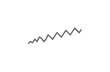
\begin{tikzpicture}[x=0.08em, y=0.08em, line width=0.4pt]
                \draw[FooterGray] (0,3) -- (1,4) -- (2,3.5) -- (3,5) -- (4,4) -- (5,6) -- (6,5.5) -- (7,4) -- (8,5) -- (9,7) -- (10,6) -- (11,5) -- (12,6.5) -- (13,8) -- (14,7) -- (15,6) -- (16,7.5) -- (17,9) -- (18,8) -- (19,7) -- (20,8.5) -- (21,10) -- (22,9) -- (23,8) -- (24,9.5);
            \end{tikzpicture}%
        }%
        \hskip0.5cm%
    }%
    \vskip6pt%
}

%=============================================================================
% PACKAGES
%=============================================================================
\usepackage[utf8]{inputenc}
\usepackage[T1]{fontenc}
\usepackage{amsmath, amssymb, amsthm}
\usepackage{mathtools}
\usepackage{bm}
\usepackage{tikz}
\usetikzlibrary{arrows.meta, positioning, shapes, calc, decorations.pathreplacing, shadings}
\usepackage{booktabs}
\usepackage{multirow}
\usepackage{array}
\usepackage{graphicx}
\usepackage{hyperref}
\usepackage{colortbl}
\hypersetup{colorlinks=true, linkcolor=MainBlue, urlcolor=MainBlue}
\graphicspath{{../../logos/}{../../charts/}}
\hfuzz=2pt

%=============================================================================
% QUANTLET COMMAND
%=============================================================================
\newcommand{\quantlet}[2]{%
    \begin{tikzpicture}[remember picture, overlay]
        \node[anchor=south east, inner sep=0pt] at ([xshift=-0.5cm, yshift=0.75cm]current page.south east) {%
            \href{#2}{%
                \raisebox{-0.1em}{\includegraphics[height=0.8em]{ql_logo.png}}%
                \textcolor{MainBlue}{\scriptsize\ #1}%
            }%
        };
    \end{tikzpicture}%
}

%=============================================================================
% CUSTOM TITLE PAGE
%=============================================================================
\defbeamertemplate*{title page}{hybrid}[1][]
{
    \vspace{0.2cm}
    % Logos row - top header (with clickable links)
    \begin{center}
        \href{https://www.ase.ro}{\includegraphics[height=1.0cm]{ase_logo.png}}\hspace{0.3cm}%
        \href{https://theida.net}{\includegraphics[height=1.0cm]{ida_logo.png}}\hspace{0.3cm}%
        \href{https://blockchain-research-center.com}{\includegraphics[height=1.0cm]{brc_logo.png}}\hspace{0.3cm}%
        \href{https://www.ai4efin.ase.ro}{\includegraphics[height=1.0cm]{ai4efin_logo.png}}\hspace{0.3cm}%
        \href{https://ipe.ro/new}{\includegraphics[height=1.0cm]{acad_logo.png}}\hspace{0.3cm}%
        \href{https://www.digital-finance-msca.com}{\includegraphics[height=1.0cm]{msca_logo.png}}%
    \end{center}

    \vspace{0.6cm}

    % Main title with Q logos on sides (with clickable links)
    \begin{center}
        \begin{minipage}{0.1\textwidth}
            \centering
            \href{https://quantlet.com}{\includegraphics[height=1.1cm]{ql_logo.png}}
        \end{minipage}%
        \begin{minipage}{0.78\textwidth}
            \centering
            {\LARGE\bfseries\usebeamercolor[fg]{title}\inserttitle}

            \vspace{0.3cm}

            {\usebeamerfont{subtitle}\usebeamercolor[fg]{title}\insertsubtitle}
        \end{minipage}%
        \begin{minipage}{0.1\textwidth}
            \centering
            \href{https://quantinar.com}{\includegraphics[height=1.1cm]{qr_logo.png}}
        \end{minipage}
    \end{center}

    \vspace{0.6cm}

    % Authors (left aligned)
    \hspace{0.5cm}{\usebeamerfont{author}\insertauthor}

    \vspace{0.3cm}

    % Institute/Affiliations (left aligned)
    \hspace{0.5cm}\begin{minipage}[t]{0.9\textwidth}
        \raggedright\small\insertinstitute
    \end{minipage}
}

%=============================================================================
% THEOREM ENVIRONMENTS
%=============================================================================
\theoremstyle{definition}
\setbeamertemplate{theorems}[numbered]
\newtheorem{defn}{Definition}
\newtheorem{thm}{Theorem}
\newtheorem{prop}{Proposition}
\newtheorem{rmk}{Remark}

%=============================================================================
% CUSTOM COMMANDS
%=============================================================================
\newcommand{\E}{\mathbb{E}}
\newcommand{\Var}{\text{Var}}
\newcommand{\Cov}{\text{Cov}}
\newcommand{\Corr}{\text{Corr}}
\newcommand{\R}{\mathbb{R}}
\newcommand{\N}{\mathbb{N}}
\newcommand{\Z}{\mathbb{Z}}
\newcommand{\RMSE}{\text{RMSE}}
\newcommand{\MAE}{\text{MAE}}
\newcommand{\MAPE}{\text{MAPE}}

%=============================================================================
% TITLE INFORMATION
%=============================================================================
\title[Time Series Analysis]{Time Series Analysis and Forecasting}
\subtitle{Chapter 8: Modern Extensions}
\author[D.T. Pele]{Daniel Traian PELE}
\institute{Bucharest University of Economic Studies\\
IDA Institute Digital Assets\\
Blockchain Research Center\\
AI4EFin Artificial Intelligence for Energy Finance\\
Romanian Academy, Institute for Economic Forecasting\\
MSCA Digital Finance}
\date{}

\begin{document}

% Title page (no header/footer)
{
\setbeamertemplate{headline}{}
\setbeamertemplate{footline}{}
\begin{frame}
    \titlepage
\end{frame}
}

%=============================================================================
% OUTLINE
%=============================================================================
\begin{frame}{Contents}
    \begin{enumerate}
        \item \textbf{Motivation} -- From Classical to Modern Methods
        \item \textbf{ARFIMA} -- Long Memory Models
        \begin{itemize}
            \item Fractional Differencing and Long Memory
            \item Estimation Methods: GPH, Local Whittle, MLE
        \end{itemize}
        \item \textbf{Random Forest} -- Ensemble Learning for Time Series
        \item \textbf{LSTM} -- Deep Learning for Sequences
        \item \textbf{Comparison} -- Model Selection Guidelines
        \item \textbf{Case Study} -- Energy Consumption Forecasting
        \item \textbf{Summary and Quiz}
    \end{enumerate}
\end{frame}

%=============================================================================
% LEARNING OBJECTIVES
%=============================================================================
\begin{frame}{Learning Objectives}
    \begin{block}{By the end of this chapter, you will be able to:}
        \begin{itemize}
            \item \textbf{Conceptual Understanding}:
            \begin{itemize}
                \item Understand long memory and fractional integration
                \item Distinguish between short and long memory processes
            \end{itemize}
            \item \textbf{Model Estimation}:
            \begin{itemize}
                \item Estimate the fractional parameter $d$ using GPH, Local Whittle, and MLE
                \item Fit and interpret ARFIMA models in Python
                \item Apply Random Forest for time series forecasting
                \item Build LSTM networks for sequential data
            \end{itemize}
            \item \textbf{Practical Skills}:
            \begin{itemize}
                \item Compare classical vs ML model performance
                \item Choose the appropriate method based on data characteristics
                \item Implement these methods in Python
            \end{itemize}
        \end{itemize}
    \end{block}
\end{frame}

%=============================================================================
\section{Motivation}
%=============================================================================

\begin{frame}{From Classical Models to Machine Learning}
    \begin{block}{The Evolution of Time Series Methods}
        \begin{itemize}
            \item \textbf{Classical ARIMA} (Box \& Jenkins, 1970) --- revolutionized forecasting but has limitations:
            \begin{itemize}
                \item Assumes \textbf{short memory}: autocorrelations decay exponentially
                \item \textbf{Linear} relationships only --- cannot capture complex dynamics
                \item Requires \textbf{stationarity} through integer differencing
            \end{itemize}
        \end{itemize}
    \end{block}

    \vspace{0.1cm}

    \begin{alertblock}{Three Paradigm Shifts}
        \begin{itemize}
            \item \textbf{ARFIMA} (Granger \& Joyeux, 1980)
            \begin{itemize}
                \item Fractional integration for long memory processes
            \end{itemize}
            \item \textbf{Random Forest} (Breiman, 2001)
            \begin{itemize}
                \item Ensemble learning for nonlinear relationships
            \end{itemize}
            \item \textbf{LSTM} (Hochreiter \& Schmidhuber, 1997)
            \begin{itemize}
                \item Deep learning for complex sequential patterns
            \end{itemize}
        \end{itemize}
    \end{alertblock}
\end{frame}

\begin{frame}{When to Use Each Method?}
    \begin{center}
    \begin{tabular}{l|c|c|c|c}
        \toprule
        \textbf{Feature} & \textbf{ARIMA} & \textbf{ARFIMA} & \textbf{RF} & \textbf{LSTM} \\
        \midrule
        Long memory & $\times$ & $\checkmark$ & $\checkmark$ & $\checkmark$ \\
        Nonlinear relationships & $\times$ & $\times$ & $\checkmark$ & $\checkmark$ \\
        Interpretability & $\checkmark$ & $\checkmark$ & $\sim$ & $\times$ \\
        Small data & $\checkmark$ & $\checkmark$ & $\times$ & $\times$ \\
        Exogenous variables & $\checkmark$ & $\checkmark$ & $\checkmark$ & $\checkmark$ \\
        Uncertainty quantification & $\checkmark$ & $\checkmark$ & $\sim$ & $\times$ \\
        \bottomrule
    \end{tabular}
    \end{center}

    \vspace{0.3cm}

    \begin{exampleblock}{Principle of Parsimony (Occam's Razor)}
        Start \textbf{simple} (ARIMA), then increase complexity only if justified by \textbf{out-of-sample} performance gains.
    \end{exampleblock}

    \vspace{0.1cm}

    {\small \textcolor{MainBlue}{\textbf{Research Evidence}}: Makridakis et al. (2018) M4 Competition showed that simple methods often outperform complex ML models on standard benchmarks.}
\end{frame}

%=============================================================================
\section{ARFIMA: Long Memory Models}
%=============================================================================

\begin{frame}{What is Long Memory?}
    \vspace{-0.2cm}
    \begin{block}{Short Memory (ARMA)}
        \begin{itemize}
            \item \textbf{ACF Behavior}:
            \begin{itemize}
                \item Autocorrelations $\rho_k$ decay \textbf{exponentially}: $|\rho_k| \leq C \cdot r^k$, $r < 1$
                \item Finite sum: $\sum_{k=0}^{\infty} |\rho_k| < \infty$
            \end{itemize}
            \item \textbf{Implication}: Shock effects disappear quickly
        \end{itemize}
    \end{block}
    \begin{alertblock}{Long Memory (ARFIMA)}
        \begin{itemize}
            \item \textbf{ACF Behavior}:
            \begin{itemize}
                \item Autocorrelations decay \textbf{hyperbolically}: $\rho_k \sim C \cdot k^{2d-1}$
                \item Infinite sum: $\sum_{k=0}^{\infty} |\rho_k| = \infty$
            \end{itemize}
            \item \textbf{Implication}: Shock effects persist for a long time
        \end{itemize}
    \end{alertblock}
    \begin{exampleblock}{Examples}
        Financial volatility, river flows, network traffic, inflation, climate data
    \end{exampleblock}
\end{frame}

\begin{frame}{Long Memory: An Intuitive Analogy}
    \begin{columns}[T]
        \begin{column}{0.48\textwidth}
            \begin{block}{Short Memory (ARMA)}
                \textbf{Analogy}: A conversation where you only remember the last few sentences.

                \vspace{0.2cm}

                \begin{itemize}
                    \item Yesterday's news? Forgotten
                    \item Last week's event? Gone
                    \item Effect of shocks fades \textbf{quickly}
                \end{itemize}

                \vspace{0.2cm}

                \textcolor{MainBlue}{\textbf{Example}}: Daily stock returns
            \end{block}
        \end{column}
        \begin{column}{0.48\textwidth}
            \begin{alertblock}{Long Memory (ARFIMA)}
                \textbf{Analogy}: An elephant that never forgets --- past events influence the present for a long time.

                \vspace{0.2cm}

                \begin{itemize}
                    \item Old shocks still matter
                    \item Slow decay of influence
                    \item \textbf{Persistent} patterns
                \end{itemize}

                \vspace{0.2cm}

                \textcolor{IDAred}{\textbf{Example}}: Stock volatility, river flows
            \end{alertblock}
        \end{column}
    \end{columns}

    \vspace{0.3cm}

    \begin{exampleblock}{Key Question}
        How fast do autocorrelations decay? \textbf{Exponentially} (short) or \textbf{hyperbolically} (long)?
    \end{exampleblock}
\end{frame}

\begin{frame}{ACF Comparison: Short Memory vs Long Memory}
    \begin{center}
        \includegraphics[width=0.95\textwidth, height=0.75\textheight, keepaspectratio]{ch8_acf_comparison.pdf}
    \end{center}
    \vspace{-0.3cm}
    {\footnotesize
    \textbf{Left}: AR(1) --- autocorrelations decay exponentially (short memory)\\
    \textbf{Right}: ARFIMA with $d=0.35$ --- autocorrelations decay hyperbolically (long memory)
    }
\quantlet{TSA\_ch8\_acf\_comparison}{https://github.com/QuantLet/TSA/tree/main/TSA_ch8/TSA_ch8_acf_comparison}
\end{frame}

\begin{frame}{The ARFIMA(p,d,q) Model}
    \begin{defn}[ARFIMA --- Granger \& Joyeux (1980), Hosking (1981)]
        A process $\{Y_t\}$ follows an \textbf{ARFIMA(p,d,q)} model if:
        $\phi(L)(1-L)^d Y_t = \theta(L)\varepsilon_t$
        where $d \in (-0.5, 0.5)$ is the \textbf{fractional differencing parameter}.
    \end{defn}

    \vspace{0.1cm}

    \begin{block}{Fractional Differencing Operator}
        $(1-L)^d = \sum_{k=0}^{\infty} \binom{d}{k}(-L)^k = 1 - dL - \frac{d(1-d)}{2!}L^2 - \frac{d(1-d)(2-d)}{3!}L^3 - \cdots$
    \end{block}

    \vspace{0.1cm}

    {\small
    \begin{itemize}
        \item $d = 0$: Standard ARMA (short memory)
        \item $0 < d < 0.5$: Long memory, stationary
        \item $d = 0.5$: Stationarity boundary
        \item $0.5 \leq d < 1$: Non-stationary, mean-reverting
        \item $d = 1$: Random walk (standard ARIMA)
    \end{itemize}
    }
\end{frame}

\begin{frame}{Interpreting the Parameter $d$}
    \begin{center}
    \begin{tabular}{c|l|l}
        \toprule
        \textbf{Value of $d$} & \textbf{ACF Behavior} & \textbf{Interpretation} \\
        \midrule
        $d = 0$ & Exponential decay & Short memory \\
        $0 < d < 0.5$ & Hyperbolic decay & Long memory, stationary \\
        $d = 0.5$ & Non-summable ACF & At the boundary \\
        $0.5 < d < 1$ & Very slow decay & Long memory, non-stationary \\
        $d = 1$ & ACF = 1 (constant) & Random walk \\
        \bottomrule
    \end{tabular}
    \end{center}

    \vspace{0.3cm}

    \begin{block}{Hurst Parameter $H$}
        Relationship with Hurst exponent: $d = H - 0.5$
        \begin{itemize}
            \item $H = 0.5$: Random walk (no memory)
            \item $H > 0.5$: Persistence (trend-following)
            \item $H < 0.5$: Anti-persistence (mean-reverting)
        \end{itemize}
    \end{block}
\end{frame}

\begin{frame}{Effect of Parameter $d$ on ACF}
    \vspace{-0.3cm}
    \begin{center}
        \includegraphics[width=0.95\textwidth, height=0.58\textheight, keepaspectratio]{ch8_arfima_d_effect.pdf}
    \end{center}
    \vspace{-0.4cm}
    {\footnotesize
    The higher $d$, the slower autocorrelations decay. As $d \to 0.5$, autocorrelations remain significant even at very large lags.
    }\hfill\quantlet{TSA\_ch8\_arfima\_d\_effect}{https://github.com/QuantLet/TSA/tree/main/TSA_ch8/TSA_ch8_arfima_d_effect}
\end{frame}

\begin{frame}{Hurst Exponent: Visual Interpretation}
    \begin{center}
        \includegraphics[width=0.88\textwidth, height=0.62\textheight, keepaspectratio]{ch8_hurst_interpretation.pdf}
    \end{center}
    \vspace{-0.2cm}
    {\footnotesize
    \textbf{H $<$ 0.5}: Series that frequently returns to mean (mean-reverting)\\
    \textbf{H = 0.5}: Random walk, unpredictable\\
    \textbf{H $>$ 0.5}: Persistent series, trends continue
    }
\quantlet{TSA\_ch8\_hurst\_interpretation}{https://github.com/QuantLet/TSA/tree/main/TSA_ch8/TSA_ch8_hurst_interpretation}
\end{frame}

\begin{frame}{Estimating the Hurst Exponent}
    \vspace{-0.2cm}
    \begin{block}{Classical Methods}
        \begin{itemize}\setlength{\itemsep}{1pt}
            \item \textbf{R/S Analysis} (Hurst, 1951): Regress $\log(R/S) = c + H \cdot \log(n)$
            \begin{itemize}\setlength{\itemsep}{0pt}
                \item Simple but sensitive to short-range dependence
            \end{itemize}
            \item \textbf{DFA} (Peng et al., 1994): Remove local trends, compute fluctuations
            \begin{itemize}\setlength{\itemsep}{0pt}
                \item Robust to non-stationarities and trends
            \end{itemize}
        \end{itemize}
    \end{block}
    \vspace{-0.1cm}
    \begin{block}{Frequency Domain Methods}
        \begin{itemize}\setlength{\itemsep}{1pt}
            \item \textbf{GPH estimator}: $\hat{d} = -\hat{\beta}/2$ from log-periodogram; $H = d + 0.5$
            \item \textbf{Wavelet-based} (Abry \& Veitch, 1998): Multi-scale decomposition, robust
        \end{itemize}
    \end{block}
\end{frame}

\begin{frame}{ARIMA vs ARFIMA: Memory Decay Patterns}
    \begin{center}
        \includegraphics[width=0.88\textwidth, height=0.62\textheight, keepaspectratio]{ch8_arima_vs_arfima.pdf}
    \end{center}
    \vspace{-0.2cm}
    {\footnotesize
    \begin{itemize}
        \item \textbf{ARIMA} (left): ACF decays \textbf{exponentially} -- shocks are quickly ``forgotten''
        \item \textbf{ARFIMA} (right, $d=0.35$): ACF decays \textbf{hyperbolically} -- shocks persist for long periods
    \end{itemize}
    }
\quantlet{TSA\_ch8\_arima\_vs\_arfima}{https://github.com/QuantLet/TSA/tree/main/TSA_ch8/TSA_ch8_arima_vs_arfima}
\end{frame}

\begin{frame}{Real Data Example: EUR/RON Long Memory Analysis}
    \vspace{-0.3cm}
    \begin{center}
        \includegraphics[width=0.95\textwidth, height=0.58\textheight, keepaspectratio]{ch8_eurron_long_memory.pdf}
    \end{center}
    \vspace{-0.4cm}
    {\footnotesize
    \textbf{Returns}: $H \approx 0.50$, $d \approx 0$ -- short memory \quad
    \textbf{Squared returns}: $H \approx 0.65$, $d \approx 0.15$ -- long memory in volatility
    }\hfill\quantlet{TSA\_ch8\_eurron\_long\_memory}{https://github.com/QuantLet/TSA/tree/main/TSA_ch8/TSA_ch8_eurron_long_memory}
\end{frame}

\begin{frame}{ARFIMA Example: S\&P 500 Realized Volatility}
    \vspace{0.3cm}
    \begin{center}
        \includegraphics[width=0.75\textwidth, height=0.38\textheight, keepaspectratio]{ch8_arfima_real_data.pdf}
    \end{center}
    \vspace{-0.1cm}
    \begin{block}{Estimation Results}
        \begin{itemize}
            \item Data: S\&P 500 (2015--2024), Hurst: $H = 0.92$, $d = H - 0.5 = 0.42$ -- strong long memory
        \end{itemize}
    \end{block}
    \begin{alertblock}{Key Insight}
        \begin{itemize}
            \item Volatility has \textbf{long memory} -- shocks persist longer than ARMA; use ARFIMA or FIGARCH!
        \end{itemize}
    \end{alertblock}
\quantlet{TSA\_ch8\_arfima\_sp500}{https://github.com/QuantLet/TSA/tree/main/TSA_ch8/TSA_ch8_arfima_sp500}
\end{frame}

\begin{frame}{ARFIMA vs ARIMA: When to Use?}
    \begin{columns}[T]
        \begin{column}{0.48\textwidth}
            \begin{block}{Use ARFIMA when:}
                \begin{itemize}
                    \item ACF decays \textbf{slowly} (hyperbolically)
                    \item $H$ significantly $\neq 0.5$
                    \item \textbf{Long horizon} forecasting
                    \item Modeling \textbf{volatility}
                \end{itemize}
            \end{block}

            \vspace{0.1cm}

            \begin{exampleblock}{Use ARIMA when:}
                \begin{itemize}
                    \item ACF decays \textbf{rapidly} (exponentially)
                    \item Short series ($< 500$ obs.)
                    \item \textbf{Short horizon} forecasting
                    \item Simplicity is priority
                \end{itemize}
            \end{exampleblock}
        \end{column}
        \begin{column}{0.48\textwidth}
            \begin{alertblock}{ARFIMA Limitations}
                \begin{itemize}
                    \item More complex estimation
                    \item Requires longer series
                    \item Estimation of $d$ is sensitive
                    \item Not always better short-term
                \end{itemize}
            \end{alertblock}

            \vspace{0.1cm}

            \begin{block}{ARFIMA Advantages}
                \begin{itemize}
                    \item Parsimonious (single $d$)
                    \item Better long-horizon forecasts
                    \item Captures slow ACF decay
                \end{itemize}
            \end{block}
        \end{column}
    \end{columns}
\end{frame}

\begin{frame}{Practical Applications of Long Memory}
    \begin{columns}[T]
        \begin{column}{0.48\textwidth}
            \begin{block}{Finance}
                \begin{itemize}
                    \item \textbf{Volatility modeling}: GARCH may underestimate persistence
                    \item \textbf{Risk management}: Long-horizon VaR
                    \item \textbf{Option pricing}: Long memory affects implied volatility
                    \item \textbf{Portfolio optimization}: Correlations persist longer
                \end{itemize}
            \end{block}
        \end{column}
        \begin{column}{0.48\textwidth}
            \begin{block}{Other Domains}
                \begin{itemize}
                    \item \textbf{Hydrology}: River flows, precipitation
                    \item \textbf{Network traffic}: Internet data packets
                    \item \textbf{Economics}: Inflation, GDP growth
                    \item \textbf{Climate}: Temperature anomalies
                    \item \textbf{Geophysics}: Earthquake magnitudes
                \end{itemize}
            \end{block}
        \end{column}
    \end{columns}

    \vspace{0.3cm}

    \begin{alertblock}{Key Insight}
        Long memory means that \textbf{shocks have lasting effects} -- important for policy, risk management, and forecasting!
    \end{alertblock}
\end{frame}

\begin{frame}{ARFIMA Estimation: Step-by-Step Procedure}
    \begin{block}{Recommended Workflow}
        \begin{enumerate}
            \item \textbf{Test for Long Memory}:
            \begin{itemize}
                \item Examine ACF decay pattern (slow = long memory)
                \item Compute $\hat{H}$ using R/S or GPH; test if $H \neq 0.5$
            \end{itemize}
            \item \textbf{Estimate $d$}:
            \begin{itemize}
                \item Use GPH or Local Whittle for initial estimate
                \item Verify $d \in (0, 0.5)$ for stationary long memory
            \end{itemize}
            \item \textbf{Fit Full ARFIMA(p,d,q)}:
            \begin{itemize}
                \item Fix $\hat{d}$ from step 2, select $p,q$ via AIC/BIC
                \item Or estimate all parameters jointly via MLE
            \end{itemize}
            \item \textbf{Diagnostic Checking}:
            \begin{itemize}
                \item Residuals should be white noise (Ljung-Box test)
                \item Check for remaining autocorrelation structure
            \end{itemize}
        \end{enumerate}
    \end{block}
\end{frame}

\begin{frame}{Real Example: Long Memory in Volatility}
    \begin{center}
        \includegraphics[width=0.98\textwidth, height=0.68\textheight, keepaspectratio]{ch8_volatility_long_memory.pdf}
    \end{center}
    \vspace{-0.3cm}
    {\footnotesize
    \textbf{Stylized Fact}: Financial returns have short memory, but volatility (|returns|) has long memory! This is the basis for FIGARCH models.
    }
\quantlet{TSA\_ch8\_volatility\_long\_memory}{https://github.com/QuantLet/TSA/tree/main/TSA_ch8/TSA_ch8_volatility_long_memory}
\end{frame}

%=============================================================================
% ARFIMA ESTIMATION METHODS
%=============================================================================

\begin{frame}{ARFIMA Estimation: Overview of Methods}
    \vspace{-0.2cm}
    \begin{block}{Three Main Approaches}
        \begin{enumerate}
            \item \textbf{GPH (Geweke-Porter-Hudak)}: Log-periodogram regression
            \begin{itemize}
                \item Semiparametric, uses only low frequencies
                \item Simple but less efficient
            \end{itemize}
            \item \textbf{Local Whittle}: Frequency-domain likelihood
            \begin{itemize}
                \item More efficient than GPH
                \item Robust to short-memory contamination
            \end{itemize}
            \item \textbf{Exact MLE (Sowell, 1992)}: Full parametric approach
            \begin{itemize}
                \item Most efficient, requires full model specification
                \item Computationally intensive
            \end{itemize}
        \end{enumerate}
    \end{block}

    \begin{alertblock}{Key Trade-off}
        \textbf{Semiparametric} (GPH, Whittle): Robust, fewer assumptions\\
        \textbf{Parametric} (MLE): More efficient, requires correct model specification
    \end{alertblock}
\end{frame}

\begin{frame}{GPH Estimator (Geweke \& Porter-Hudak, 1983)}
    \begin{defn}[Log-Periodogram Regression]
        The GPH estimator is based on the regression:
        \[
        \ln I(\omega_j) = c - d \ln\left(4\sin^2\left(\frac{\omega_j}{2}\right)\right) + \text{error}
        \]
        where $I(\omega_j)$ is the periodogram at Fourier frequency $\omega_j = \frac{2\pi j}{n}$.
    \end{defn}

    \vspace{0.1cm}

    \begin{block}{Key Properties}
        \begin{itemize}
            \item Uses only \textbf{lowest $m$ frequencies} where long-memory dominates
            \item Typical choice: $m = n^{0.5}$ to $n^{0.8}$ (trade-off bias vs variance)
            \item \textbf{Asymptotic normality}: $\sqrt{m}(\hat{d} - d) \xrightarrow{d} N(0, \frac{\pi^2}{24})$
            \item Simple OLS regression, easy to implement
        \end{itemize}
    \end{block}

    \begin{alertblock}{Bandwidth Selection}
        Too small $m$: High variance \quad Too large $m$: Bias from short-memory component
    \end{alertblock}
\end{frame}

\begin{frame}{Local Whittle Estimator (Robinson, 1995)}
    \begin{defn}[Local Whittle Objective Function]
        The Local Whittle estimator minimizes:
        \[
        R(d) = \ln\left(\frac{1}{m}\sum_{j=1}^{m} \omega_j^{2d} I(\omega_j)\right) - \frac{2d}{m}\sum_{j=1}^{m} \ln(\omega_j)
        \]
        where $m$ is the bandwidth parameter.
    \end{defn}

    \vspace{0.1cm}

    \begin{block}{Advantages over GPH}
        \begin{itemize}
            \item \textbf{More efficient}: Lower asymptotic variance than GPH
            \item \textbf{Asymptotic normality}: $\sqrt{m}(\hat{d} - d) \xrightarrow{d} N(0, \frac{1}{4})$
            \item Robust to \textbf{additive noise} and \textbf{mean shifts}
            \item Does not require periodogram smoothing
        \end{itemize}
    \end{block}

    \begin{exampleblock}{Practical Note}
        Both GPH and Local Whittle are \textbf{semiparametric}: they estimate $d$ without specifying the short-memory (ARMA) structure.
    \end{exampleblock}
\end{frame}

\begin{frame}{Exact MLE: Sowell (1992)}
    \begin{block}{Full Parametric Approach}
        The exact MLE maximizes the Gaussian log-likelihood:
        \[
        \ell(\phi, d, \theta, \sigma^2) = -\frac{n}{2}\ln(2\pi\sigma^2) - \frac{1}{2}\ln|\Sigma| - \frac{1}{2\sigma^2}\mathbf{y}'\Sigma^{-1}\mathbf{y}
        \]
        where $\Sigma$ is the autocovariance matrix of the ARFIMA(p,d,q) process.
    \end{block}

    \vspace{0.1cm}

    \begin{columns}[T]
        \begin{column}{0.48\textwidth}
            \begin{exampleblock}{Advantages}
                \begin{itemize}
                    \item \textbf{Most efficient} (achieves Cram\'{e}r-Rao bound)
                    \item Joint estimation of $d$, $\phi$, $\theta$
                    \item Standard errors for all parameters
                \end{itemize}
            \end{exampleblock}
        \end{column}
        \begin{column}{0.48\textwidth}
            \begin{alertblock}{Disadvantages}
                \begin{itemize}
                    \item Requires \textbf{correct model specification}
                    \item \textbf{Computationally intensive} ($O(n^3)$)
                    \item Sensitive to non-Gaussianity
                \end{itemize}
            \end{alertblock}
        \end{column}
    \end{columns}

    \vspace{0.2cm}

    {\small \textbf{Sowell's contribution}: Efficient algorithm to compute exact autocovariances of ARFIMA.}
\end{frame}

\begin{frame}{Approximate MLE Methods}
    \begin{block}{Computational Alternatives to Exact MLE}
        \begin{itemize}
            \item \textbf{CSS (Conditional Sum of Squares)}:
            \begin{itemize}
                \item Conditions on initial values, avoids matrix inversion
                \item Fast but less efficient for small samples
            \end{itemize}
            \item \textbf{Whittle Likelihood}:
            \begin{itemize}
                \item Frequency-domain approximation: $\ell_W = -\sum_j \left[\ln f(\omega_j) + \frac{I(\omega_j)}{f(\omega_j)}\right]$
                \item $O(n \log n)$ complexity via FFT
            \end{itemize}
            \item \textbf{State-Space Representation}:
            \begin{itemize}
                \item Kalman filter for likelihood evaluation
                \item Handles missing data naturally
            \end{itemize}
        \end{itemize}
    \end{block}

    \begin{exampleblock}{Practical Recommendation}
        For large samples ($n > 1000$): Use Whittle or CSS\\
        For small samples ($n < 500$): Use exact MLE if feasible
    \end{exampleblock}
\end{frame}

\begin{frame}[fragile]{ARFIMA Estimation in Python}
    \vspace{-0.2cm}
    \begin{block}{Using the \texttt{arch} Package (Approximate MLE)}
\begin{verbatim}
from arch.univariate import ARFIMA
import numpy as np

# Estimate ARFIMA(1,d,1) with d estimated
model = ARFIMA(returns, p=1, d=None, q=1)
result = model.fit()

# Display results
print(f"Estimated d: {result.params['d']:.4f}")
print(f"Std Error:   {result.std_err['d']:.4f}")
print(f"95% CI: [{result.params['d'] - 1.96*result.std_err['d']:.4f}, "
      f"{result.params['d'] + 1.96*result.std_err['d']:.4f}]")
\end{verbatim}
    \end{block}

    \vspace{-0.1cm}

    {\footnotesize
    \begin{alertblock}{Key Points}
        \begin{itemize}
            \item \texttt{d=None}: Estimate $d$ from data \quad \texttt{d=0.3}: Fix $d$ at 0.3
            \item Uses approximate MLE (efficient for moderate samples)
            \item Also available: \texttt{statsmodels.tsa.arima.model.ARIMA} with \texttt{trend='n'}
        \end{itemize}
    \end{alertblock}
    }
\quantlet{TSA\_ch8\_arfima\_estimation}{https://github.com/QuantLet/TSA/tree/main/TSA_ch8/TSA_ch8_arfima_estimation}
\end{frame}

\begin{frame}[fragile]{GPH and Hurst Estimation in Python}
    \vspace{-0.3cm}
    \begin{block}{Semiparametric Estimation}
\begin{verbatim}
from statsmodels.tsa.stattools import acf
from hurst import compute_Hc  # pip install hurst
import numpy as np

# Method 1: Hurst exponent via R/S analysis
H, c, data = compute_Hc(returns, kind='price')
d_rs = H - 0.5
print(f"Hurst (R/S): {H:.4f}, d = {d_rs:.4f}")

# Method 2: GPH estimator (simplified)
def gph_estimator(y, m=None):
    n = len(y)
    m = m or int(n**0.5)
    from scipy.fft import fft
    I = np.abs(fft(y - np.mean(y)))**2 / (2*np.pi*n)
    j = np.arange(1, m+1)
    omega = 2*np.pi*j/n
    x = np.log(4*np.sin(omega/2)**2)
    y_reg = np.log(I[1:m+1])
    d_hat = -np.polyfit(x, y_reg, 1)[0]
    return d_hat
\end{verbatim}
    \end{block}
\quantlet{TSA\_ch8\_gph\_estimation}{https://github.com/QuantLet/TSA/tree/main/TSA_ch8/TSA_ch8_gph_estimation}
\end{frame}

\begin{frame}{Comparing Estimation Methods: Summary}
    \vspace{-0.2cm}
    \begin{center}
    {\small
    \begin{tabular}{l|c|c|c|c}
        \toprule
        \textbf{Method} & \textbf{Efficiency} & \textbf{Robustness} & \textbf{Speed} & \textbf{Assumptions} \\
        \midrule
        GPH & Low & High & Fast & Minimal \\
        Local Whittle & Medium & High & Fast & Minimal \\
        Whittle MLE & Medium-High & Medium & Medium & Parametric \\
        Exact MLE & Highest & Low & Slow & Full model \\
        \bottomrule
    \end{tabular}
    }
    \end{center}

    \vspace{0.2cm}

    \begin{block}{Recommended Workflow}
        \begin{enumerate}
            \item \textbf{Initial screening}: Use GPH or Hurst exponent to detect long memory
            \item \textbf{Robust estimation}: Use Local Whittle to estimate $d$
            \item \textbf{Final model}: Fit ARFIMA(p,d,q) via MLE with $\hat{d}$ as starting value
            \item \textbf{Validation}: Compare different bandwidths/methods for robustness
        \end{enumerate}
    \end{block}

    \begin{alertblock}{Sensitivity Check}
        If GPH and Whittle estimates differ substantially, investigate short-memory contamination or structural breaks.
    \end{alertblock}
\end{frame}

%=============================================================================
\section{Random Forest for Time Series}
%=============================================================================

\begin{frame}{Random Forest: Basic Concepts}
    \begin{block}{What is Random Forest? (Breiman, 2001)}
        \begin{itemize}
            \item \textbf{Ensemble learning} method combining multiple decision trees:
            \begin{itemize}
                \item Each tree trained on a \textbf{bootstrap sample} (bagging)
                \item At each split, only $m \ll p$ \textbf{random features} considered
                \item Final prediction = \textbf{average} of all tree predictions
            \end{itemize}
        \end{itemize}
    \end{block}

    \vspace{0.1cm}

    \begin{exampleblock}{Why It Works for Time Series}
        \begin{itemize}
            \item \textbf{Flexibility}:
            \begin{itemize}
                \item Captures nonlinear relationships and interactions automatically
                \item No stationarity assumption required
            \end{itemize}
            \item \textbf{Robustness}:
            \begin{itemize}
                \item Resistant to outliers, noise, and irrelevant features
                \item Built-in feature importance for interpretability
            \end{itemize}
        \end{itemize}
    \end{exampleblock}
\end{frame}

\begin{frame}{Why ``Random'' Forest? The Power of Diversity}
    \begin{block}{Two Sources of Randomness}
        \begin{enumerate}
            \item \textbf{Bootstrap Sampling}: Each tree sees a different subset of data
            \item \textbf{Feature Sampling}: Each split considers only $m$ random features
        \end{enumerate}
    \end{block}

    \vspace{0.2cm}

    \begin{columns}[T]
        \begin{column}{0.48\textwidth}
            \begin{exampleblock}{Analogy: Wisdom of Crowds}
                \begin{itemize}
                    \item Ask 100 people to guess weight of an ox
                    \item Individual guesses: high variance
                    \item \textbf{Average}: remarkably accurate!
                \end{itemize}
            \end{exampleblock}
        \end{column}
        \begin{column}{0.48\textwidth}
            \begin{alertblock}{Why It Works}
                \begin{itemize}
                    \item Trees make \textbf{different errors}
                    \item Errors \textbf{cancel out} when averaging
                    \item Result: lower variance, same bias
                \end{itemize}
            \end{alertblock}
        \end{column}
    \end{columns}

    \vspace{0.3cm}

    \begin{block}{Mathematical Insight}
        If trees are uncorrelated with variance $\sigma^2$, forest variance = $\frac{\sigma^2}{B}$ (B = number of trees)
    \end{block}
\end{frame}

\begin{frame}{How Does a Decision Tree Make Predictions?}
    \begin{columns}[T]
        \begin{column}{0.55\textwidth}
            \begin{center}
            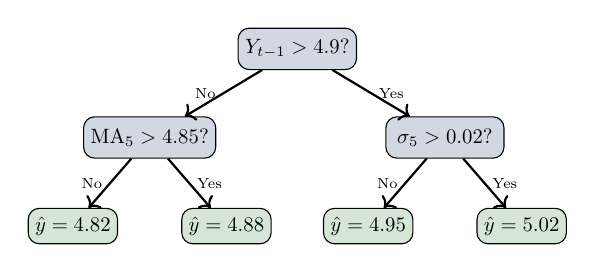
\begin{tikzpicture}[scale=0.75, transform shape,
                node/.style={draw, rectangle, rounded corners, fill=MainBlue!20, minimum width=2cm, minimum height=0.7cm, align=center},
                leaf/.style={draw, rectangle, rounded corners, fill=Forest!20, minimum width=1.5cm, minimum height=0.6cm, align=center},
                edge/.style={->, thick}]

                % Root node
                \node[node] (root) at (0,0) {$Y_{t-1} > 4.9$?};

                % Level 1
                \node[node] (l1) at (-2.5,-1.5) {$\text{MA}_5 > 4.85$?};
                \node[node] (r1) at (2.5,-1.5) {$\sigma_5 > 0.02$?};

                % Leaves
                \node[leaf] (ll) at (-3.8,-3) {$\hat{y}=4.82$};
                \node[leaf] (lr) at (-1.2,-3) {$\hat{y}=4.88$};
                \node[leaf] (rl) at (1.2,-3) {$\hat{y}=4.95$};
                \node[leaf] (rr) at (3.8,-3) {$\hat{y}=5.02$};

                % Edges
                \draw[edge] (root) -- node[left, font=\scriptsize] {No} (l1);
                \draw[edge] (root) -- node[right, font=\scriptsize] {Yes} (r1);
                \draw[edge] (l1) -- node[left, font=\scriptsize] {No} (ll);
                \draw[edge] (l1) -- node[right, font=\scriptsize] {Yes} (lr);
                \draw[edge] (r1) -- node[left, font=\scriptsize] {No} (rl);
                \draw[edge] (r1) -- node[right, font=\scriptsize] {Yes} (rr);
            \end{tikzpicture}
            \end{center}
        \end{column}
        \begin{column}{0.43\textwidth}
            \begin{block}{Tree Prediction}
                \begin{enumerate}
                    \item Start at the root
                    \item Check the condition (split)
                    \item Go left (No) or right (Yes)
                    \item Repeat until a leaf
                    \item \textbf{Leaf value = prediction}
                \end{enumerate}
            \end{block}

            \begin{exampleblock}{Random Forest}
                $\hat{y} = \frac{1}{B}\sum_{b=1}^{B} T_b(\mathbf{x})$ --- Average of $B$ trees
            \end{exampleblock}
        \end{column}
    \end{columns}
\end{frame}

\begin{frame}{Random Forest: Mathematical Formulation}
    \vspace{-0.3cm}
    \begin{block}{Prediction}
        $\hat{y} = \frac{1}{B} \sum_{b=1}^{B} T_b(\mathbf{x})$ \quad where $T_b(\mathbf{x})$ = prediction of tree $b$
    \end{block}

    \vspace{-0.1cm}

    \begin{block}{Feature Importance (MDI = Mean Decrease in Impurity)}
        $\text{Importance}(X_j) = \frac{1}{B} \sum_{b=1}^{B} \sum_{\substack{t \in T_b \\ j_t = j}} \Delta I_t$

        {\small Sum over all nodes $t$ in all trees where feature $j$ was used; $\Delta I_t$ = impurity decrease}
    \end{block}

    \vspace{-0.1cm}

    \begin{block}{Out-of-Bag Error (OOB)}
        $\text{OOB} = \frac{1}{n} \sum_{i=1}^{n} L\left(y_i, \frac{1}{|B_i^{-}|} \sum_{b \in B_i^{-}} T_b(\mathbf{x}_i)\right)$

        {\small $B_i^{-}$ = trees where obs. $i$ was \textbf{not} in the bootstrap (free validation!)}
    \end{block}
\end{frame}

\begin{frame}{Random Forest: How It Works}
    \begin{columns}[T]
        \begin{column}{0.55\textwidth}
            \begin{block}{Training Process}
                \begin{enumerate}
                    \item Draw $B$ bootstrap samples
                    \item For each sample $b$, grow tree $T_b$:
                    \begin{itemize}
                        \item At each node, select $m$ features
                        \item Find best split: $\min_{j,s} \sum (y_i - \bar{y}_{R_1})^2$
                        \item Continue until stopping criterion
                    \end{itemize}
                    \item Aggregate: $\hat{y} = \frac{1}{B}\sum_{b=1}^B T_b(\mathbf{x})$
                \end{enumerate}
            \end{block}
        \end{column}
        \begin{column}{0.43\textwidth}
            \begin{alertblock}{Key Hyperparameters}
                \begin{itemize}
                    \item $B$: number of trees (100-500)
                    \item $m$: features per split ($\sqrt{p}$)
                    \item max\_depth: tree depth
                    \item min\_samples: leaf size
                \end{itemize}
            \end{alertblock}
        \end{column}
    \end{columns}
\end{frame}

\begin{frame}{Feature Engineering: The Key to ML Success}
    \vspace{-0.2cm}
    \begin{alertblock}{Critical Insight}
        ML models don't ``understand'' time --- you must \textbf{encode temporal patterns as features}!
    \end{alertblock}
    \vspace{-0.1cm}
    \begin{columns}[T]
        \begin{column}{0.48\textwidth}
            \begin{block}{Lag Features}
                {\small $y_{t-1}, y_{t-2}, \ldots$ -- capture \textbf{AR} patterns}
            \end{block}
            \begin{block}{Rolling Statistics}
                {\small Mean $\bar{y}_{k,t}$, std $\sigma_{k,t}$ -- \textbf{local trends}}
            \end{block}
        \end{column}
        \begin{column}{0.48\textwidth}
            \begin{block}{Calendar Features}
                {\small Day, month, holiday -- \textbf{seasonality}}
            \end{block}
            \begin{exampleblock}{Domain Features}
                {\small Weather, economics -- external \textbf{regressors}}
            \end{exampleblock}
        \end{column}
    \end{columns}
    \quantlet{TSA\_ch8\_feature\_engineering}{https://github.com/QuantLet/TSA/tree/main/TSA_ch8/TSA_ch8_feature_engineering}
\end{frame}

\begin{frame}{Random Forest: Why It Works for Time Series}
    \vspace{-0.2cm}
    \begin{columns}[T]
        \begin{column}{0.48\textwidth}
            \begin{block}{Strengths}
                \begin{itemize}\setlength{\itemsep}{2pt}
                    \item No linearity assumption
                    \item Automatic interaction detection
                    \item Handles mixed data types
                    \item Built-in OOB validation
                    \item Parallelizable training
                \end{itemize}
            \end{block}
        \end{column}
        \begin{column}{0.48\textwidth}
            \begin{alertblock}{Limitations}
                \begin{itemize}\setlength{\itemsep}{2pt}
                    \item Cannot extrapolate beyond training range
                    \item Requires manual feature engineering
                    \item Less interpretable than single tree
                \end{itemize}
            \end{alertblock}
        \end{column}
    \end{columns}
\end{frame}

%=============================================================================
\section{LSTM: Deep Learning for Time Series}
%=============================================================================

\begin{frame}{From Biological to Artificial Neurons}
    \vspace{0.3cm}
    \begin{center}
        \includegraphics[width=0.75\textwidth, height=0.38\textheight, keepaspectratio]{ch8_neuron_comparison.pdf}
    \end{center}
    \vspace{-0.1cm}
    \begin{block}{The Analogy}
        \begin{itemize}
            \item \textbf{Dendrites} $\rightarrow$ \textbf{Inputs} $x_i$ \quad \textbf{Synapses} $\rightarrow$ \textbf{Weights} $w_i$ \quad \textbf{Soma} $\rightarrow$ \textbf{Sum + Activation} \quad \textbf{Axon} $\rightarrow$ \textbf{Output} $y$
        \end{itemize}
    \end{block}
    \quantlet{TSA\_ch8\_neuron\_comparison}{https://github.com/QuantLet/TSA/tree/main/TSA_ch8/TSA_ch8_neuron_comparison}
\end{frame}

\begin{frame}{Recurrent Neural Networks (RNN)}
    \vspace{-0.3cm}
    \begin{center}
        \includegraphics[width=0.85\textwidth, height=0.38\textheight, keepaspectratio]{ch8_rnn_unfolded.pdf}
    \end{center}
    \vspace{-0.3cm}
    \begin{columns}[T]
        \begin{column}{0.48\textwidth}
            \begin{block}{Key Idea}
                \begin{itemize}\setlength{\itemsep}{2pt}
                    \item Processes \textbf{sequences} step by step
                    \item Hidden state $h_t$ carries \textbf{memory}
                    \item Update: $h_t = \tanh(W_h h_{t-1} + W_x x_t)$
                \end{itemize}
            \end{block}
        \end{column}
        \begin{column}{0.50\textwidth}
            \begin{alertblock}{Vanishing Gradient Problem}
                \begin{itemize}\setlength{\itemsep}{2pt}
                    \item \textbf{Gradient}: derivative to update weights
                    \item Long sequences: $\frac{\partial L}{\partial h_1} \propto \prod W_h \to 0$
                    \item Early steps \textbf{stop learning}
                    \item \textbf{Solution}: LSTM/GRU gates
                \end{itemize}
            \end{alertblock}
        \end{column}
    \end{columns}
\quantlet{TSA\_ch8\_rnn\_unfolded}{https://github.com/QuantLet/TSA/tree/main/TSA_ch8/TSA_ch8_rnn_unfolded}
\end{frame}

\begin{frame}{LSTM: Long Short-Term Memory}
    \vspace{-0.2cm}
    \begin{block}{The LSTM Solution (Hochreiter \& Schmidhuber, 1997)}
        A gated architecture with \textbf{3 learned gates} that control information flow:
        \textbf{Forget} ($f_t$) -- what to discard; \textbf{Input} ($i_t$) -- what to store; \textbf{Output} ($o_t$) -- what to transmit
    \end{block}

    \vspace{-0.1cm}

    \begin{block}{LSTM Equations}
        {\footnotesize
        \begin{align*}
            f_t &= \sigma(W_f \cdot [h_{t-1}, x_t] + b_f) & \text{(Forget)} \\
            i_t &= \sigma(W_i \cdot [h_{t-1}, x_t] + b_i) & \text{(Input)} \\
            \tilde{C}_t &= \tanh(W_C \cdot [h_{t-1}, x_t] + b_C) & \text{(Candidate)} \\
            C_t &= f_t \odot C_{t-1} + i_t \odot \tilde{C}_t & \text{(Cell state)} \\
            o_t &= \sigma(W_o \cdot [h_{t-1}, x_t] + b_o) & \text{(Output)} \\
            h_t &= o_t \odot \tanh(C_t) & \text{(Hidden state)}
        \end{align*}
        }
    \end{block}
\end{frame}

\begin{frame}{LSTM Gates: An Intuitive Explanation}
    \begin{block}{Analogy: A Smart Secretary}
        The LSTM cell is like a secretary managing information flow in an office.
    \end{block}

    \vspace{0.2cm}

    \begin{columns}[T]
        \begin{column}{0.32\textwidth}
            \begin{alertblock}{Forget Gate $f_t$}
                \textbf{``What to throw away?''}

                \vspace{0.1cm}

                \begin{itemize}
                    \item Reviews old files
                    \item Decides what's outdated
                    \item $f_t \approx 0$: delete
                    \item $f_t \approx 1$: keep
                \end{itemize}
            \end{alertblock}
        \end{column}
        \begin{column}{0.32\textwidth}
            \begin{block}{Input Gate $i_t$}
                \textbf{``What to file?''}

                \vspace{0.1cm}

                \begin{itemize}
                    \item Reviews new info
                    \item Decides importance
                    \item $i_t \approx 0$: ignore
                    \item $i_t \approx 1$: store
                \end{itemize}
            \end{block}
        \end{column}
        \begin{column}{0.32\textwidth}
            \begin{exampleblock}{Output Gate $o_t$}
                \textbf{``What to report?''}

                \vspace{0.1cm}

                \begin{itemize}
                    \item Reviews memory
                    \item Decides relevance
                    \item $o_t \approx 0$: hide
                    \item $o_t \approx 1$: share
                \end{itemize}
            \end{exampleblock}
        \end{column}
    \end{columns}
    \vspace{0.1cm}
    \begin{block}{Key Insight}
        Gates are \textbf{learned} during training --- the network discovers what to remember and forget!
    \end{block}
\end{frame}

\begin{frame}{LSTM Cell Architecture}
    \vspace{-0.2cm}
    \begin{center}
        \includegraphics[width=0.88\textwidth, height=0.52\textheight, keepaspectratio]{ch8_lstm_cell.pdf}
    \end{center}
    \vspace{-0.4cm}
    {\footnotesize
    \textbf{Cell State} ($C_t$): Long-term memory \quad
    \textbf{Hidden State} ($h_t$): Short-term memory \quad
    \textbf{Gates}: \textcolor{IDAred}{forget}, \textcolor{Forest}{add}, \textcolor{AccentBlue}{transmit}
    }
\quantlet{TSA\_ch8\_lstm\_cell}{https://github.com/QuantLet/TSA/tree/main/TSA_ch8/TSA_ch8_lstm_cell}
\end{frame}

\begin{frame}{Activation Functions: Why Do We Need Them?}
    \vspace{0.3cm}
    \begin{center}
        \includegraphics[width=0.75\textwidth, height=0.38\textheight, keepaspectratio]{ch8_activation_functions.pdf}
    \end{center}
    \vspace{-0.1cm}
    \begin{block}{Why Activation Functions?}
        \begin{itemize}
            \item Without them, networks can only learn \textbf{linear} relationships
            \item \textbf{In LSTM}: Sigmoid for gates (0-1), Tanh for cell state (-1 to 1)
        \end{itemize}
    \end{block}
\end{frame}

\begin{frame}{LSTM Advantages for Time Series}
    \vspace{-0.2cm}
    \begin{columns}[T]
        \begin{column}{0.48\textwidth}
            \begin{exampleblock}{Why LSTM?}
                \begin{itemize}\setlength{\itemsep}{2pt}
                    \item Captures long-term dependencies
                    \item Variable-length sequences
                    \item Complex nonlinear patterns
                    \item Multivariate time series
                \end{itemize}
            \end{exampleblock}
        \end{column}
        \begin{column}{0.48\textwidth}
            \begin{alertblock}{Disadvantages}
                \begin{itemize}\setlength{\itemsep}{2pt}
                    \item Needs large datasets
                    \item ``Black box'' model
                    \item Sensitive to hyperparameters
                    \item Prone to overfitting
                \end{itemize}
            \end{alertblock}
        \end{column}
    \end{columns}
\end{frame}

\begin{frame}{LSTM: Key Hyperparameters}
    \begin{columns}[T]
        \begin{column}{0.48\textwidth}
            \begin{block}{Architecture}
                \begin{itemize}
                    \item \textbf{Units}: neurons per layer (32-256)
                    \item \textbf{Layers}: stacked LSTM (1-3)
                    \item \textbf{Sequence length}: past observations (10-100)
                    \item \textbf{Dropout}: regularization (0.1-0.3)
                \end{itemize}
            \end{block}
        \end{column}
        \begin{column}{0.48\textwidth}
            \begin{block}{Training}
                \begin{itemize}
                    \item \textbf{Batch size}: samples per update (32-128)
                    \item \textbf{Epochs}: training iterations (50-200)
                    \item \textbf{Learning rate}: step size (0.001)
                    \item \textbf{Early stopping}: prevents overfitting
                \end{itemize}
            \end{block}
        \end{column}
    \end{columns}

    \vspace{0.3cm}

    \begin{alertblock}{Practical Tips}
        \begin{itemize}
            \item \textbf{Normalize/scale} data to [0,1] or [-1,1]
            \item Use \textbf{validation set} for hyperparameter tuning
            \item Monitor \textbf{training vs validation loss} for overfitting
        \end{itemize}
    \end{alertblock}
\end{frame}

\begin{frame}{LSTM: When to Use It}
    \begin{block}{LSTM is a Good Choice When:}
        \begin{itemize}
            \item \textbf{Data Characteristics}:
            \begin{itemize}
                \item Large datasets ($>$ 1000 observations)
                \item Complex temporal patterns and long-term dependencies
            \end{itemize}
            \item \textbf{Problem Requirements}:
            \begin{itemize}
                \item Multiple input sequences (multivariate)
                \item Accuracy is more important than interpretability
            \end{itemize}
        \end{itemize}
    \end{block}

    \begin{alertblock}{LSTM is NOT a Good Choice When:}
        \begin{itemize}
            \item \textbf{Data Limitations}:
            \begin{itemize}
                \item Small datasets ($<$ 500 obs) or linear relationships
            \end{itemize}
            \item \textbf{Practical Constraints}:
            \begin{itemize}
                \item Interpretable predictions required
                \item Limited computational resources
                \item Simple models (ARIMA) already perform well
            \end{itemize}
        \end{itemize}
    \end{alertblock}
\end{frame}

%=============================================================================
\section{Comparison and Model Selection}
%=============================================================================

\begin{frame}{Evaluation Metrics}
    \vspace{-0.2cm}
    {\small \textbf{Notation}: $y_i$ = actual value, $\hat{y}_i$ = predicted value, $n$ = number of observations}
    \vspace{0.1cm}
    \begin{block}{Common Metrics}
        \begin{itemize}
            \item \textbf{Scale-Dependent}:
            \begin{itemize}
                \item RMSE: $\sqrt{\frac{1}{n}\sum(y_i - \hat{y}_i)^2}$ --- penalizes large errors
                \item MAE: $\frac{1}{n}\sum|y_i - \hat{y}_i|$ --- robust to outliers
            \end{itemize}
            \item \textbf{Scale-Free}:
            \begin{itemize}
                \item MAPE: $\frac{100}{n}\sum\left|\frac{y_i - \hat{y}_i}{y_i}\right|$ --- percentage error
                \item MASE: $\frac{\text{MAE}}{\frac{1}{n-1}\sum_{i=2}^{n}|y_i - y_{i-1}|}$ --- relative to naive (random walk)
            \end{itemize}
        \end{itemize}
    \end{block}

    \begin{alertblock}{Validation for Time Series}
        \begin{itemize}
            \item \textbf{Critical}: Do NOT use standard k-fold cross-validation!
            \begin{itemize}
                \item Use Time Series CV (walk-forward validation)
                \item Or temporal train/validation/test split
            \end{itemize}
        \end{itemize}
    \end{alertblock}
\end{frame}

\begin{frame}{Time Series Cross-Validation}
    \begin{center}
        \includegraphics[width=0.92\textwidth, height=0.68\textheight, keepaspectratio]{ch8_timeseries_cv.pdf}
    \end{center}
    \vspace{-0.2cm}
    {\footnotesize
    \textbf{Important}: Training set grows progressively; test is always in the future $\Rightarrow$ avoids data leakage.
    }
\quantlet{TSA\_ch8\_timeseries\_cv}{https://github.com/QuantLet/TSA/tree/main/TSA_ch8/TSA_ch8_timeseries_cv}
\end{frame}

\begin{frame}{Model Selection Guide}
    \vspace{-0.3cm}
    \begin{center}
    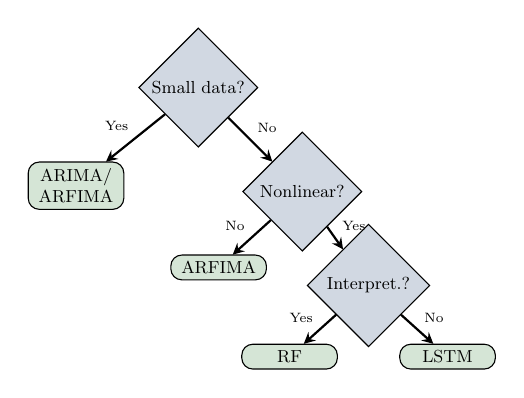
\begin{tikzpicture}[scale=0.7, transform shape,
        node distance=1cm,
        decision/.style={diamond, draw, fill=MainBlue!20, text width=1.8cm, align=center, inner sep=1pt, font=\small},
        block/.style={rectangle, draw, fill=Forest!20, text width=1.5cm, align=center, rounded corners, font=\small},
        arrow/.style={thick,->,>=stealth}
    ]
        \node[decision] (start) {Small data?};
        \node[block, below left=0.8cm and 0.8cm of start] (arima) {ARIMA/ ARFIMA};
        \node[decision, below right=0.8cm and 0.8cm of start] (nonlin) {Nonlinear?};
        \node[block, below left=0.6cm and 0.1cm of nonlin] (arfima) {ARFIMA};
        \node[decision, below right=0.6cm and 0.1cm of nonlin] (interp) {Interpret.?};
        \node[block, below left=0.5cm and 0cm of interp] (rf) {RF};
        \node[block, below right=0.5cm and 0cm of interp] (lstm) {LSTM};

        \draw[arrow] (start) -- node[above left, font=\scriptsize] {Yes} (arima);
        \draw[arrow] (start) -- node[above right, font=\scriptsize] {No} (nonlin);
        \draw[arrow] (nonlin) -- node[above left, font=\scriptsize] {No} (arfima);
        \draw[arrow] (nonlin) -- node[above right, font=\scriptsize] {Yes} (interp);
        \draw[arrow] (interp) -- node[above left, font=\scriptsize] {Yes} (rf);
        \draw[arrow] (interp) -- node[above right, font=\scriptsize] {No} (lstm);
    \end{tikzpicture}
    \end{center}
    \vspace{-0.1cm}
    {\small
    \begin{alertblock}{Trade-off}
        ML models offer better accuracy but higher computational cost. For small data or interpretability, ARIMA/ARFIMA remain excellent choices.
    \end{alertblock}
    }
\end{frame}

%=============================================================================
% KEY FORMULAS SUMMARY
%=============================================================================
\begin{frame}{Key Formulas -- Summary}
    \vspace{-0.2cm}
    {\small
    \begin{columns}[T]
        \begin{column}{0.48\textwidth}
            \begin{block}{ARFIMA(p,d,q)}
                $\phi(L)(1-L)^d Y_t = \theta(L)\varepsilon_t$

                \vspace{0.1cm}
                {\footnotesize $d \in (-0.5, 0.5)$: long memory}
            \end{block}

            \begin{block}{Long Memory}
                ACF: $\rho_k \sim C \cdot k^{2d-1}$

                Hurst: $d = H - 0.5$

                \vspace{0.1cm}
                {\footnotesize $H > 0.5$: persistence}
            \end{block}

            \begin{block}{Random Forest}
                $\hat{y} = \frac{1}{B}\sum_{b=1}^{B} T_b(x)$

                \vspace{0.1cm}
                {\footnotesize $B$ trees, random features}
            \end{block}
        \end{column}

        \begin{column}{0.48\textwidth}
            \begin{block}{LSTM Cell}
                $f_t = \sigma(W_f[h_{t-1}, x_t] + b_f)$

                $C_t = f_t \odot C_{t-1} + i_t \odot \tilde{C}_t$

                \vspace{0.1cm}
                {\footnotesize Forget, Input, Output gates}
            \end{block}

            \begin{block}{Evaluation Metrics}
                RMSE $= \sqrt{\frac{1}{n}\sum(y_i - \hat{y}_i)^2}$

                MAPE $= \frac{100}{n}\sum\left|\frac{y_i - \hat{y}_i}{y_i}\right|$
            \end{block}

            \begin{block}{Time Series CV}
                Walk-forward validation

                Train $\rightarrow$ Test (temporal split)
            \end{block}
        \end{column}
    \end{columns}
    }
\end{frame}

%=============================================================================
\section{Case Study: Energy Consumption}
%=============================================================================

\begin{frame}{Case Study: Energy Consumption Forecasting}
    \begin{columns}[T]
        \begin{column}{0.55\textwidth}
            \begin{block}{Data Source}
                \begin{itemize}
                    \item \textbf{Series}: Germany daily electricity consumption
                    \item \textbf{Unit}: Gigawatt-hours (GWh)
                    \item \textbf{Period}: Jan 2012 -- Dec 2017
                    \item \textbf{Observations}: 2,162 daily values
                    \item \textbf{Source}: Open Power System Data
                \end{itemize}
            \end{block}

            \begin{alertblock}{Data Split (Temporal!)}
                \begin{itemize}
                    \item \textbf{Training}: 70\% (1,513 obs)
                    \item \textbf{Validation}: 15\% (324 obs)
                    \item \textbf{Test}: 15\% (325 obs)
                \end{itemize}
            \end{alertblock}
        \end{column}
        \begin{column}{0.43\textwidth}
            \begin{exampleblock}{Key Patterns}
                \begin{itemize}
                    \item \textbf{Weekly}: Lower on weekends
                    \item \textbf{Annual}: Higher in winter
                    \item \textbf{Holidays}: Significant drops
                    \item \textbf{Trend}: Slight decrease
                \end{itemize}
            \end{exampleblock}

            \vspace{0.1cm}

            {\footnotesize
            \textbf{Why ML works here:}\\
            Complex multi-seasonal patterns + sufficient data (2000+ obs) = ideal for ML!
            }
        \end{column}
    \end{columns}
\end{frame}

\begin{frame}{Case Study: Feature Engineering}
    \vspace{-0.2cm}
    \begin{columns}[T]
        \begin{column}{0.48\textwidth}
            \begin{block}{Lag Features}
                \begin{itemize}\setlength{\itemsep}{2pt}
                    \item Previous day: $y_{t-1}$
                    \item Same day last week: $y_{t-7}$
                    \item Two weeks ago: $y_{t-14}$
                    \item Full week history: $y_{t-1}, \ldots, y_{t-7}$
                \end{itemize}
            \end{block}
            \begin{block}{Rolling Statistics}
                \begin{itemize}\setlength{\itemsep}{2pt}
                    \item 7-day mean: $\bar{y}_{7,t} = \frac{1}{7}\sum_{i=1}^{7} y_{t-i}$
                    \item 7-day std: $\sigma_{7,t}$
                    \item 30-day mean: $\bar{y}_{30,t}$
                \end{itemize}
            \end{block}
        \end{column}
        \begin{column}{0.48\textwidth}
            \begin{block}{Calendar Features}
                \begin{itemize}\setlength{\itemsep}{2pt}
                    \item Day of week (1--7)
                    \item Month (1--12)
                    \item Is weekend (0/1)
                    \item Is holiday (0/1)
                \end{itemize}
            \end{block}
            \begin{alertblock}{Avoid Data Leakage!}
                \begin{itemize}\setlength{\itemsep}{2pt}
                    \item Use \textbf{only past data}
                    \item Rolling stats: exclude $y_t$
                    \item Scale with \textbf{training} stats only
                \end{itemize}
            \end{alertblock}
        \end{column}
    \end{columns}
    \vspace{0.1cm}
    {\small \textbf{Total: 14 features} for Random Forest and LSTM models}
\end{frame}

\begin{frame}{Case Study: Models Compared}
    \vspace{-0.2cm}
    {\small
    \begin{center}
    \begin{tabular}{l|l|l}
        \toprule
        \textbf{Model} & \textbf{Description} & \textbf{Configuration} \\
        \midrule
        \textbf{Baseline} & Seasonal naive: $\hat{y}_t = y_{t-7}$ & No parameters \\
        \midrule
        \textbf{SARIMA} & Seasonal ARIMA with & Order: $(1,1,1)$ \\
         & weekly seasonality & Seasonal: $(1,0,1)_7$ \\
        \midrule
        \textbf{ARFIMA} & Fractional differencing & $H = 0.77 \Rightarrow d = 0.27$ \\
         & with long memory & Rolling one-step forecasts \\
        \midrule
        \textbf{Random} & Ensemble of 200 trees & max\_depth = 15 \\
        \textbf{Forest} & with all 14 features & min\_samples\_leaf = 5 \\
        \midrule
        \textbf{LSTM} & 2-layer LSTM (64, 32 units) & seq\_length = 7 days \\
         & with all 14 features & dropout = 0.2, early stopping \\
        \bottomrule
    \end{tabular}
    \end{center}
    }

    \vspace{0.2cm}

    \begin{exampleblock}{Evaluation Metric: MAPE}
        $\text{MAPE} = \frac{100}{n}\sum_{i=1}^{n}\left|\frac{y_i - \hat{y}_i}{y_i}\right|$ --- interpretable as ``average \% error''
    \end{exampleblock}
\end{frame}

\begin{frame}{Case Study: Data Overview}
    \begin{center}
        \includegraphics[width=0.98\textwidth, height=0.75\textheight, keepaspectratio]{ch8_data_split.pdf}
    \end{center}
    \vspace{-0.3cm}
    {\small
    \textbf{Train}: 1513 obs (70\%) \quad \textbf{Validation}: 324 obs (15\%) \quad \textbf{Test}: 325 obs (15\%)
    }
\quantlet{TSA\_ch8\_data\_split}{https://github.com/QuantLet/TSA/tree/main/TSA_ch8/TSA_ch8_data_split}
\end{frame}

\begin{frame}{Case Study: Model Predictions}
    \begin{center}
        \includegraphics[width=0.98\textwidth, height=0.52\textheight, keepaspectratio]{ch8_model_predictions.pdf}
    \end{center}
    \vspace{-0.3cm}
    {\footnotesize
    \begin{center}
    \begin{tabular}{l|c|c|l}
        \textbf{Rank} & \textbf{Model} & \textbf{MAPE} & \textbf{Interpretation} \\
        \hline
        1 & \textcolor{Forest}{\textbf{Random Forest}} & \textcolor{Forest}{\textbf{2.2\%}} & Best: captures nonlinear patterns \\
        2 & \textcolor{IDAred}{\textbf{LSTM}} & \textcolor{IDAred}{\textbf{3.3\%}} & Good, needs more data \\
        3 & \textcolor{AccentBlue}{\textbf{Baseline}} & \textcolor{AccentBlue}{\textbf{3.9\%}} & Simple but competitive \\
        4 & \textcolor{Orange}{\textbf{ARFIMA}} & \textcolor{Orange}{\textbf{12.3\%}} & Long memory not sufficient \\
        5 & \textcolor{Purple}{\textbf{SARIMA}} & \textcolor{Purple}{\textbf{14.6\%}} & Struggles with patterns \\
    \end{tabular}
    \end{center}
    }
\quantlet{TSA\_ch8\_model\_predictions}{https://github.com/QuantLet/TSA/tree/main/TSA_ch8/TSA_ch8_model_predictions}
\end{frame}

\begin{frame}{Case Study: Best Model Performance}
    \vspace{-0.3cm}
    \begin{center}
        \includegraphics[width=0.90\textwidth, height=0.55\textheight, keepaspectratio]{ch8_best_model_prediction.pdf}
    \end{center}
    \vspace{-0.3cm}
    \begin{columns}[T]
        \begin{column}{0.46\textwidth}
            \begin{block}{Random Forest Wins}
                \begin{itemize}\setlength{\itemsep}{1pt}
                    \item MAPE: \textbf{2.2\%}
                    \item Captures weekly patterns
                \end{itemize}
            \end{block}
        \end{column}
        \begin{column}{0.46\textwidth}
            \begin{alertblock}{Why RF Outperformed?}
                \begin{itemize}\setlength{\itemsep}{1pt}
                    \item Good feature engineering
                    \item Robust to outliers
                \end{itemize}
            \end{alertblock}
        \end{column}
    \end{columns}
\quantlet{TSA\_ch8\_best\_model}{https://github.com/QuantLet/TSA/tree/main/TSA_ch8/TSA_ch8_best_model}
\end{frame}

%=============================================================================
\begin{frame}{Practical Summary: Model Selection}
    \begin{center}
    \begin{tabular}{l|c|c|c|c}
        \toprule
        \textbf{Criterion} & \textbf{ARIMA} & \textbf{ARFIMA} & \textbf{RF} & \textbf{LSTM} \\
        \midrule
        Data needed & Few & Few & Medium & Many \\
        Long memory & No & \textbf{Yes} & Partial & Partial \\
        Nonlinearity & No & No & \textbf{Yes} & \textbf{Yes} \\
        Interpretability & \textbf{Yes} & \textbf{Yes} & Partial & No \\
        Computation time & Fast & Fast & Medium & Slow \\
        Exog. variables & Limited & Limited & \textbf{Yes} & \textbf{Yes} \\
        \bottomrule
    \end{tabular}
    \end{center}
    \vspace{0.2cm}
    {\small \textbf{Rule}: Start simple (ARIMA), increase complexity only if out-of-sample performance improves.}
\end{frame}

\begin{frame}{Common Mistakes to Avoid}
    \begin{columns}[T]
        \begin{column}{0.48\textwidth}
            \begin{alertblock}{Data Leakage}
                \begin{itemize}
                    \item Using future data in features
                    \item Standard k-fold CV on time series
                    \item Scaling with full dataset stats
                \end{itemize}
                \textbf{Solution}: Always use \textbf{walk-forward} validation
            \end{alertblock}

            \begin{alertblock}{Overfitting}
                \begin{itemize}
                    \item Too many features
                    \item Too complex models
                    \item Training too long (LSTM)
                \end{itemize}
                \textbf{Solution}: Use \textbf{validation set}, early stopping
            \end{alertblock}
        \end{column}
        \begin{column}{0.48\textwidth}
            \begin{alertblock}{Wrong Model Choice}
                \begin{itemize}
                    \item LSTM with 100 observations
                    \item ARIMA for nonlinear patterns
                    \item Ignoring interpretability needs
                \end{itemize}
                \textbf{Solution}: Match model to \textbf{data size \& complexity}
            \end{alertblock}

            \begin{alertblock}{Poor Evaluation}
                \begin{itemize}
                    \item Only using RMSE
                    \item Ignoring prediction intervals
                    \item No baseline comparison
                \end{itemize}
                \textbf{Solution}: Multiple metrics, \textbf{always compare to naive}
            \end{alertblock}
        \end{column}
    \end{columns}
\end{frame}

\begin{frame}{Practical Workflow: Step-by-Step}
    \begin{center}
    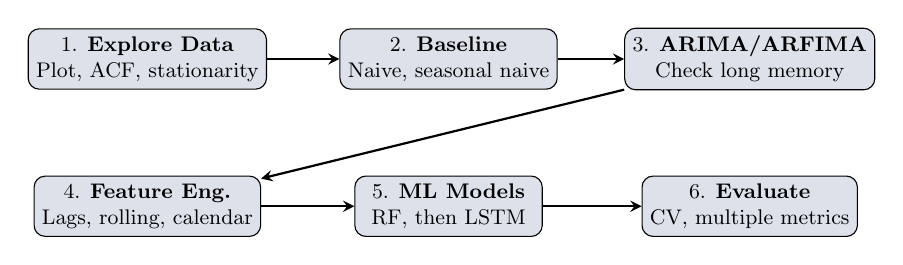
\begin{tikzpicture}[scale=0.85, transform shape,
        box/.style={draw, rectangle, rounded corners, fill=MainBlue!15, minimum width=2.8cm, minimum height=0.9cm, align=center, font=\small},
        arrow/.style={->, thick, >=stealth}]

        % Step 1
        \node[box] (s1) at (0,0) {1. \textbf{Explore Data}\\Plot, ACF, stationarity};

        % Step 2
        \node[box] (s2) at (4.5,0) {2. \textbf{Baseline}\\Naive, seasonal naive};

        % Step 3
        \node[box] (s3) at (9,0) {3. \textbf{ARIMA/ARFIMA}\\Check long memory};

        % Step 4
        \node[box] (s4) at (0,-2.2) {4. \textbf{Feature Eng.}\\Lags, rolling, calendar};

        % Step 5
        \node[box] (s5) at (4.5,-2.2) {5. \textbf{ML Models}\\RF, then LSTM};

        % Step 6
        \node[box] (s6) at (9,-2.2) {6. \textbf{Evaluate}\\CV, multiple metrics};

        % Arrows
        \draw[arrow] (s1) -- (s2);
        \draw[arrow] (s2) -- (s3);
        \draw[arrow] (s3) -- (s4);
        \draw[arrow] (s4) -- (s5);
        \draw[arrow] (s5) -- (s6);

    \end{tikzpicture}
    \end{center}

    \vspace{0.3cm}

    \begin{exampleblock}{Golden Rules}
        \begin{itemize}
            \item \textbf{Start simple}: Beat the baseline first, then add complexity
            \item \textbf{Validate properly}: Time series CV, not random splits
            \item \textbf{Iterate}: Feature engineering often matters more than model choice
        \end{itemize}
    \end{exampleblock}
\end{frame}

%=============================================================================
\section{Summary and Quiz}
%=============================================================================

\begin{frame}{Summary}
    \begin{block}{What We Learned}
        \begin{itemize}\setlength{\itemsep}{3pt}
            \item \textbf{ARFIMA}: Extends ARIMA for long memory processes (fractional $d$)
            \item \textbf{Random Forest}: Ensemble of trees for nonlinear relationships
            \item \textbf{LSTM}: Deep learning for complex sequential dependencies
            \item \textbf{Trade-offs}: Complexity vs interpretability vs data requirements
        \end{itemize}
    \end{block}
    \vspace{0.2cm}
    \begin{exampleblock}{Key Takeaway}
        \begin{itemize}
            \item \textbf{Parsimony Principle}:
            \begin{itemize}
                \item Simple models often outperform complex ones
                \item Always benchmark against naive methods
            \end{itemize}
        \end{itemize}
    \end{exampleblock}
\end{frame}

\begin{frame}{Quick Quiz}
    \begin{enumerate}\setlength{\itemsep}{8pt}
        \item What does $d = 0.3$ mean in an ARFIMA model?
        \item Why use Time Series CV instead of standard k-fold?
        \item What is the main advantage of LSTM over simple RNNs?
        \item What type of model would you choose with small data and linear relationships?
        \item What does ``data leakage'' mean in the context of ML for time series?
    \end{enumerate}
\end{frame}

\begin{frame}{Quiz Answers}
    {\small
    \begin{enumerate}
        \item \textbf{$d = 0.3$}: Long memory, the series is stationary but autocorrelations decay slowly (hyperbolically). Moderate persistence.

        \vspace{0.15cm}

        \item \textbf{Time Series CV}: To respect temporal order. Standard k-fold would use future data to predict the past (data leakage).

        \vspace{0.15cm}

        \item \textbf{LSTM vs RNN}: LSTM solves the ``vanishing gradient'' problem through the gating mechanism, allowing learning of long-term dependencies.

        \vspace{0.15cm}

        \item \textbf{Small data, linear relationships}: ARIMA or ARFIMA. ML requires lots of data to generalize well.

        \vspace{0.15cm}

        \item \textbf{Data leakage}: Using future information in features or training. E.g., calculating moving averages using future data, or standard k-fold that mixes temporal order.
    \end{enumerate}
    }
\end{frame}

\begin{frame}{What Comes Next?}
    \begin{block}{Chapter 9: Multiple Seasonalities}
        \begin{itemize}
            \item \textbf{The Challenge}: Real data often has multiple seasonal patterns
            \begin{itemize}
                \item Hourly data: daily + weekly + yearly cycles
                \item Standard SARIMA handles only one seasonal period
            \end{itemize}
            \item \textbf{TBATS}: Trigonometric seasonality, Box-Cox, ARMA errors, Trend, Seasonal
            \begin{itemize}
                \item Automatic, handles high-frequency data
                \item Uses Fourier terms for efficient representation
            \end{itemize}
            \item \textbf{Prophet} (Taylor \& Letham, 2018): Decomposable model
            \begin{itemize}
                \item Interpretable components (trend + seasonality + holidays)
                \item Built-in holiday effects and external regressors
            \end{itemize}
        \end{itemize}
    \end{block}

    \begin{center}
        \Large\textcolor{MainBlue}{Questions?}
    \end{center}
\end{frame}

\begin{frame}{Key References}
    \vspace{-0.2cm}
    {\footnotesize
    \begin{block}{Foundational Papers}
        \begin{itemize}
            \item Box, G.E.P. \& Jenkins, G.M. (1970). \textit{Time Series Analysis: Forecasting and Control}. Holden-Day.
            \item Granger, C.W.J. \& Joyeux, R. (1980). An introduction to long-memory time series models and fractional differencing. \textit{Journal of Time Series Analysis}, 1(1), 15-29.
            \item Hosking, J.R.M. (1981). Fractional differencing. \textit{Biometrika}, 68(1), 165-176.
        \end{itemize}
    \end{block}

    \begin{block}{Machine Learning Methods}
        \begin{itemize}
            \item Breiman, L. (2001). Random Forests. \textit{Machine Learning}, 45(1), 5-32.
            \item Hochreiter, S. \& Schmidhuber, J. (1997). Long short-term memory. \textit{Neural Computation}, 9(8), 1735-1780.
        \end{itemize}
    \end{block}

    \begin{block}{Forecasting Competitions \& Reviews}
        \begin{itemize}
            \item Makridakis, S., Spiliotis, E. \& Assimakopoulos, V. (2018). The M4 Competition. \textit{International Journal of Forecasting}, 34(4), 802-808.
            \item Hyndman, R.J. \& Athanasopoulos, G. (2021). \textit{Forecasting: Principles and Practice}, 3rd ed. OTexts.
        \end{itemize}
    \end{block}
    }
\end{frame}

%=============================================================================
% SUMMARY
%=============================================================================
\section{Summary}

\begin{frame}{Key Takeaways}
\begin{block}{What We Learned}
\begin{itemize}
    \item ARFIMA captures long memory with fractional differencing parameter $d \in (0, 0.5)$
    \item Random Forests and LSTM offer flexible alternatives when traditional models fail
    \item Time series cross-validation is essential to prevent data leakage
\end{itemize}
\end{block}

\begin{alertblock}{Important}
Feature engineering often matters more than model complexity. Always benchmark against simple methods (naive, seasonal naive). The Hurst exponent helps detect long memory before modeling.
\end{alertblock}
\end{frame}

\end{document}
